\section{Δίκτυα \& Μηχανισμοί Κωδικοποίησης 3D Εισόδου \\ DeepSDF Frequency Feature Embeddings}
\label{section:dnnEmbeddings}
Στο πλαίσιο της καλύτερης δυνατής ανακατασκευής \enit{3D} γραφικών όσον αφορά την ακρίβεια του σήματος που ισοδυναμεί με την αποτύπωση
υψηλοσυχνοτικών περιοχών  εισάγεται η έννοια των δικτύων κωδικοποίησης. Αυτός είναι η βασική μεθοδολογία με την οποία δίνεται η δυνατότητα η εκπαίδευση των νευρωνικά ελεγχόμενων διαφορίσιμων ισομετρικών επιφανειών (\enit{Neural Level Sets}) να μπορέσει να συλλάβει υψηλοσυχνοτικό περιεχόμενο.  Επομένως, η βάση της διπλωματικής είναι οι τρισδιάστατες κωδικοποιήσεις 3D πληροφορίας με χρήση βαθιών νευρωνικών δικτύων που αναλύονται παρακάτω. 

\subsection{Κωδικοποίηση μέσω συναρτήσεων εφαπτόμενου νευρωνικού πυρήνα Fourier - Fourier Feature Neural Tangent Kernel}
\par
    Παρά του θεωρήματος γενικευμένης δυνατότητας αναπαράστασης συναρτήσεων από πλήρως συνδεδεμένα γραμμικά δίκτυα MLP (ακόμα και μονο-στρωματικά), τα τεχνητά νευρωνικά δίκτυα στην πραγματικότητα δεν μπορούν να ανταποκριθούν πλήρως σε αυτήν την ιδιότητα. Θεωρητικά πρέπει να ισχύουν, οριακές συνθήκες που προβλέπουν να υπάρχει άπειρο πλήθος νευρώνων στο στρώμα, ενώ το βήμα εκπαίδευσης στον αλγόριθμο βελτιστοποίησης για παράδειγμα SGD να (\enit{Stochastic Gradient Descent}) τείνει στο 0. Αυτό το πρόβλημα καλούνται να λύσουν εξειδικευμένες συναρτήσεις βελτιστοποίησης, τεχνικές αποκοπής νευρώνων αλλά ακόμα και ειδική προ επεξεργασία δεδομένων που ωστόσο αποτυγχάνουν μιας και δεν καταφέρνουν να συλλάβουν τις σχέσεις δεδομένων σε ανώτερες διαστάσεις. Σε αυτό το πλαίσιο επιδρούν πυρήνες συναρτήσεων ή δίκτυα κωδικοποίησης που μετασχηματίζουν την είσοδο εισάγοντας ποιοτικά χαρακτηριστικά που σχετίζονται με την έξοδο προς αναπαράσταση κάνοντας αντιστοίχηση των εισόδων των δικτύων σε χώρους μεγαλύτερης διάστασης ή με ιδιαίτερα χαρακτηριστικά. 
    \begin{figure}[ht]
        \centering
        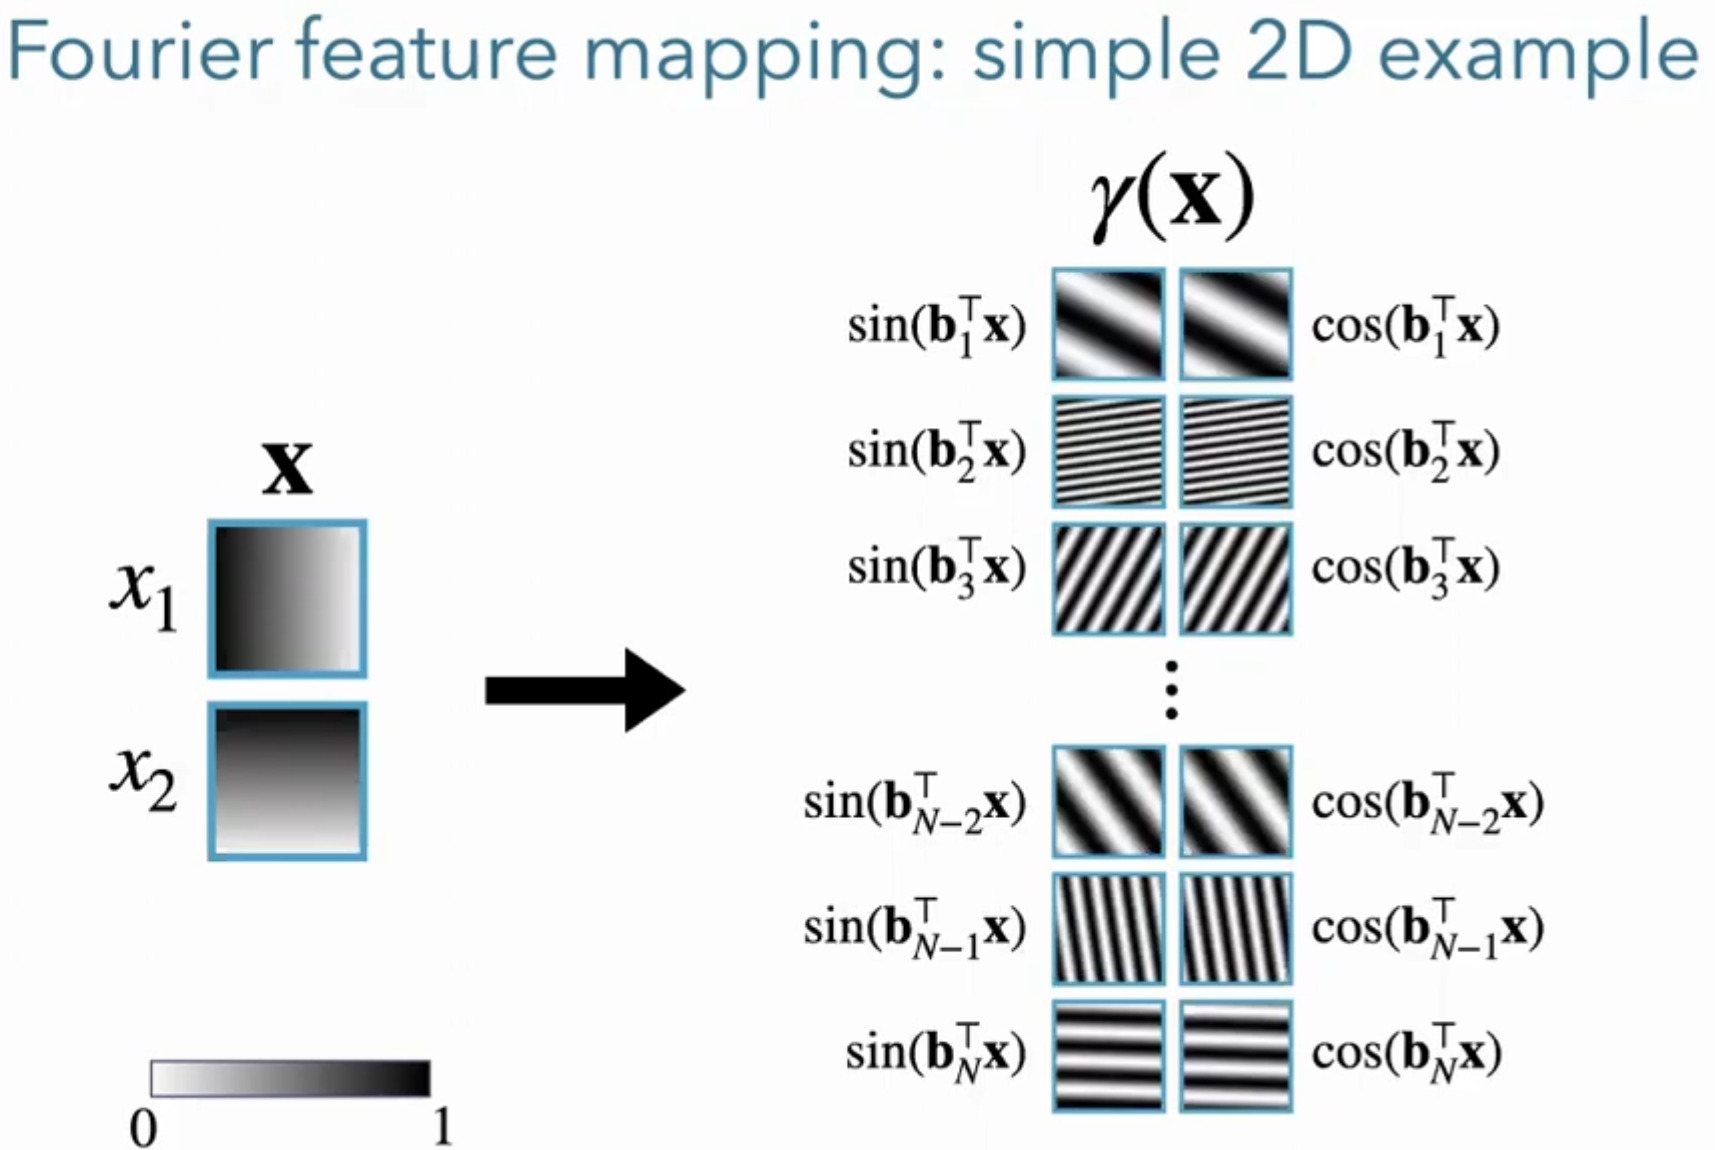
\includegraphics[width=.4\linewidth]{images/chapter2_img/FourierMapping.jpg}
        \caption{Οπτική Παρουσίαση Εφαρμογής Fourier Feature Mapping σε Δισδιάστατες Εικόνες. Πηγή:(\cite{tancik2020fourier})}
        \label{fig:2dfouriermapping}
    \end{figure}
\par
    Παρατηρώντας το Σχήμα \ref{fig:2dfouriermapping}, γίνεται αντιληπτό το πως λειτουργεί ένας εφαπτόμενος πυρήνας Fourier συχνοτικής κωδικοποίησης εισόδου. Στα πλαίσια των νευρωνικών δικτύων αυτό που πρακτικά εφαρμόζεται στην συνέχεια είναι μια παλινδρόμηση πυρήνα ώστε να γίνει εκπαίδευση των ενσωματωμένων συχνοτήτων που διαθέτει πλέον η κωδικοποιημένη είσοδος. Σημαντικό ρόλο σε αυτό το κομμάτι παίζει το εύρος των συναρτήσεων πυρήνα. Σε περίπτωση που το εύρος είναι πολύ μεγάλο παρατηρείται αξιόπιστη, αλλά πολύ ομαλοποιημένη απόδοση χαρακτηριστικών ενώ σε μικρό εύρος συναρτήσεων πυρήνα παρατηρούνται φαινόμενα μη σωστής παλινδρόμησης και συνεπώς μη συνεπής ανακατασκευή που προέρχεται από φαινόμενα υπερεκπαίδευσης σε συγκεκριμένα χαρακτηριστικά.
    \begin{figure}[ht]
        \centering
        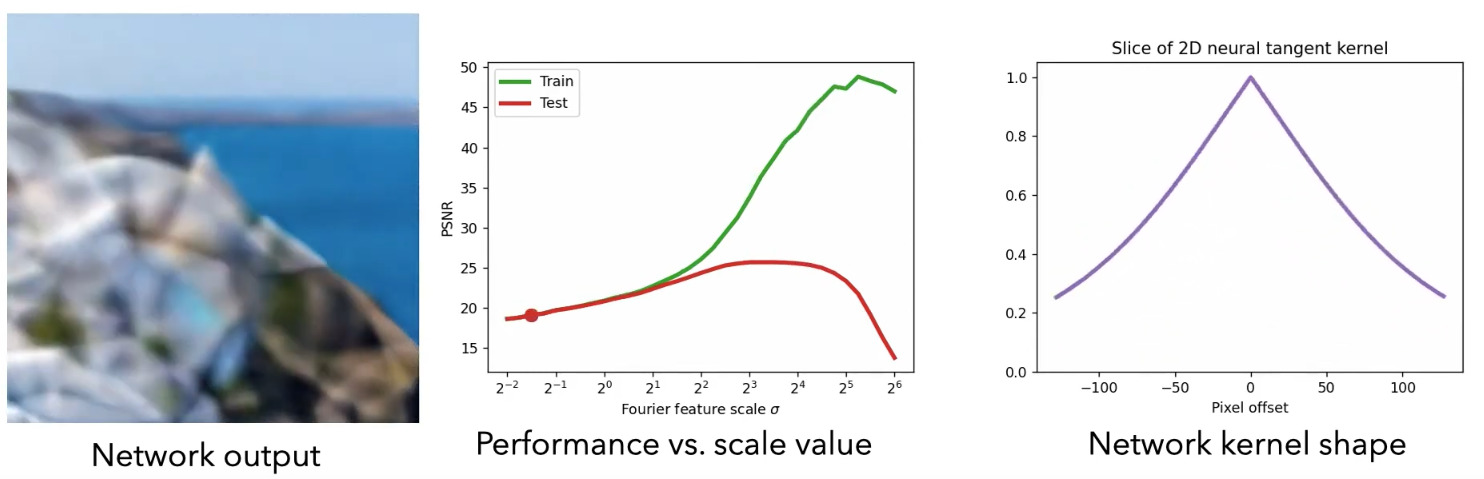
\includegraphics[width = .8\linewidth]{images/chapter2_img/WideTangentKernel.jpg}
        \caption{Ανακατασκευή εικόνας με Κωδικοποίηση Ευρύ Εφαπτόμενου Πυρήνα Συναρτήσεων Fourier (μεγάλο $\sigma$ κατανομής δειγματοληψίας συχνοτήτων),Πηγή \cite{tancik2020fourier}}
        \label{fig:wideNTK}
    \end{figure} \\
    \begin{figure}[H]
        \centering
        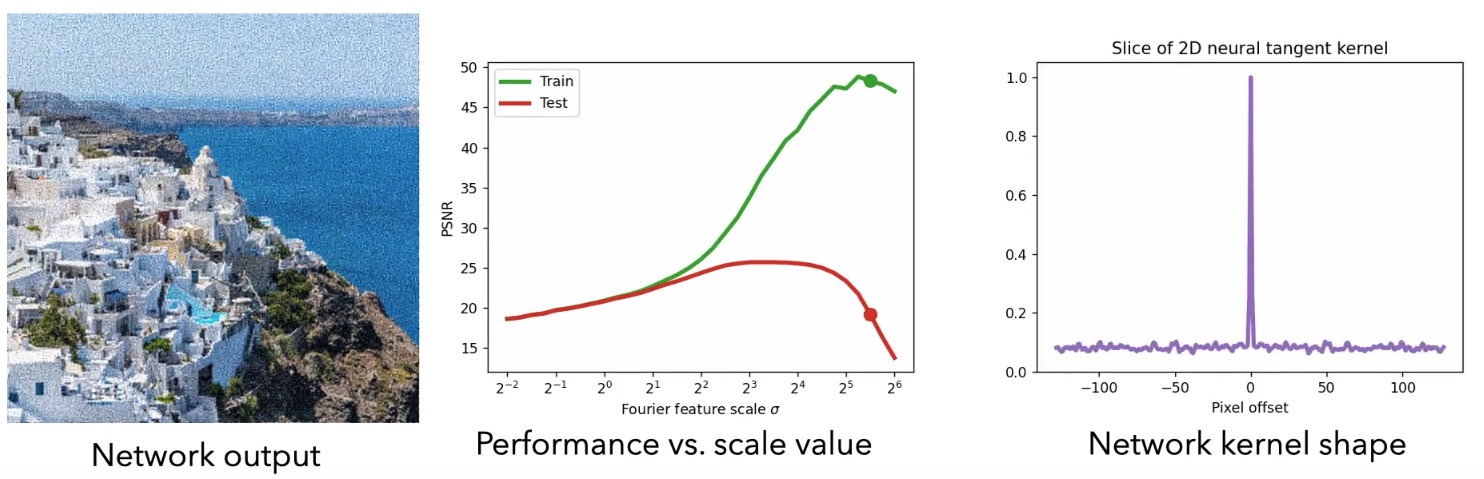
\includegraphics[width = .8\linewidth]{images/chapter2_img/NarrowTangentKernel.jpg}
        \caption{Ανακατασκευή εικόνας με Κωδικοποίηση Στενού Εφαπτόμενου Πυρήνα Συναρτήσεων Fourier (μικρό $\sigma$), Πηγή \cite{tancik2020fourier}}
        \label{fig:narrowNTK}
    \end{figure}
    Αυτή η τεχνική μπορεί να χρησιμοποιηθεί και σε τρισδιάστατη κωδικοποίηση πληροφορίας (τρισδιάστατα σημεία εισόδου, τρισδιάστατα διανύσματα κατεύθυνσης όψης) και επιφέρει ανάλογα αποτελέσματα στις έμμεσες αναπαραστάσεις που δημιουργούνται τόσο στο κομμάτι της απόδοσης χρώματος όσο και στην γεωμετρική απόδοση. 
    
\subsection{Χρήση χωρικής πληροφορίας στον εφαπτόμενο νευρωνικό πυρήνα συναρτήσεων - Positional Encoding}
\par 
    Μια ειδική κατηγορία της παραπάνω μεθόδου κωδικοποίησης είναι το \textit{Positional Encoding}. Η πρώτη εφαρμογή αυτού γίνεται στα πλαίσια της κωδικοποίησης της εισόδου σε μηχανισμού προσοχής σε δίκτυα που αφορούν την ερμηνεία φυσικής γλώσσας (\enit{Natural Language Processing}).  Στον τομέα της εργασίας πρώτη φορά αυτού του είδους η κωδικοποίηση της εισόδου εφαρμόστηκε σε δίκτυα που μαθαίνουν την ακτινοβολία μιας σκηνής \enit{Neural Radiance Fields} \cite{tancik2020fourier}.

    H παλινδρόμηση πυρήνα ή χρήση συναρτήσεων πυρήνα σε νευρωνικά δίκτυα παλινδρόμησης είναι μια συνήθης τακτική. Ωστόσο, αυτή η μέθοδος έχει πολλά να προσφέρει και ως ένα τρόπο διαμεσολάβησης σε γραμμικά δίκτυα MLP που δεν είναι πολλές φορές σε θέση να καταγράψουν συχνοτικό περιεχόμενο, ειδικά όταν αυτά τα δίκτυα είναι δίκτυα συντεταγμένων (\enit{coordinate based networks}). Όπως είναι και τα βαθιά δίκτυα SDF.  

    Έστω $f$ να αναπαριστά ένα πλήρως συνδεδεμένο νευρωνικό δίκτυο με βάρη $\theta$ που είναι αρχικοποιημένα σε με βάση μια Γκαουσιανή κατανομή Ν.  

    Το εύρος των στρωμάτων, δηλαδή το πλήθος νευρώνων τείνει στο άπειρο και το βήμα εκμάθησης στον αλγόριθμο back propagation που βελτιστοποιεί τα βάρη να τείνει στο 0. 

    Όταν συμβαίνει αυτό, οι  συναρτήσεις τύπου $f(\chi;\theta)$  συγκλίνουν κατά την διάρκεια της εκπαίδευσης κάτι το οποίο προσομοιώνει, παλινδρόμηση πυρήνα ή καλύτερα \enit{kernel regression} που αναλογεί στην χρήση ενός εφαπτόμενου νευρωνικού δικτύου με συναρτήσεις πυρήνα, (\enit{NTK Neural (Stationary) Tangent Kernel}): $$ K_{ntk}(x\_i;x\_j) = E_{\theta \sim N}<\frac{\partial{f(x\_i;\theta)}}{\partial{\theta}},\frac{\partial{f(x\_j;\theta)}}{\partial{\theta}}>$$
    Όταν οι είσοδοι είναι περιορισμένες σε μια υπερσφαίρα, ο εφαπτόμενος νευρωνικός πυρήνας για ένα MLP δίκτυο μπορεί να γραφτεί ως το εσωτερικό γινόμενο πυρήνα ($h_{NTK}(x\_i^{T}x\_j)$, όπου το $h_{NTK}:\mathbb{R}\rightarrow\mathbb{R}$ είναι βαθμωτό μέγεθος)


\subsubsection{Χρήση των Χαρακτηριστικών Fourier για τον υπολογισμό εφαπτόμενου πυρήνα κωδικοποίησης}
\par
    Η εκτίμηση μιας ακατέργαστης στάσιμης συνάρτησης πυρήνα με το θεώρημα Bocher's (Θεώρημα \ref{theorem: Bocher's Theorem}) είναι εφικτή με υψηλότερη ακρίβεια.
    Για την διαδικασία αυτή χρησιμοποιείται αντιστοίχηση της εισόδου σε χαρακτηριστικά Fourier $\gamma$ για να δοθεί στις συντεταγμένες εισόδου, συχνοτικό χαρακτηριστικό εμφάνισης, πριν να οδηγηθούν στο βασικό δίκτυο MLP που αναλαμβάνει την την αντιστοίχηση τους πάνω σε ισομετρίες.
\par
    Συγκεκριμένα η συνάρτηση $\gamma$ αντιστοιχεί τα δεδομένα εισόδου, που είναι ένα διάνυσμα $\vec{v}\in[0,1)^d$, σε ισομετρική επιφάνεια μια υψηλότερου βαθμού και στην περίπτωση της εργασίας μια υπερσφαίρα (λόγω και έμμεσης γεωμετρικής ομαλοποίησης δικτύου SDF \cite{gropp2020implicit}) με ένα σύνολο ημιτονoειδών συναρτήσεων που επηρεάζονται από ένα παράγοντα κλίμακας ή βάρους $\alpha$.
        $$\gamma\vec(v) = [\alpha_1\cdot\cos(2 \pi b_1^{T}v), \alpha_2\cdot\sin(2\pi b_2^{T}v)],....,\alpha_m\cdot\cos(2\pi b_m^{T}v)]^{T} $$
\par 
    Επειδή από την βασική τριγωνομετρία, $\cos(\alpha - \beta) = cosa\cdot cosb - sina \cdot sinb$  αυτή  η συνάρτηση πυρήνα και η κωδικοποίηση που συνεπάγεται εισάγει στις συντεταγμένες τον εξής μετασχηματισμό:
    $$K_{\gamma} = \gamma(v_1)^{T}\cdot \gamma(v_2) = \sum_{j=1}^{m}{a^2_{j}cos(2\pi b_j^{T}(v_1 - v_2)}) = h_{\gamma}(v_1-v_2)$$
    που αποτελεί μια στάσιμη εφαρμογή πυρήνα κωδικοποίησης Fourier, δηλαδή μια συνάρτηση που διατηρεί την ισομετρική ιδιότητα των δεδομένων και είναι αμετάβλητη σε περιστροφές ή μετατοπίσεις μιας και είναι κωδικοποίηση που αφορά μόνο την απόσταση των σημείων για αυτό αποκαλείται και κωδικοποίηση τοπολογική ή positional encoding. 
\par
    Με την χρήση αυτής την κωδικοποίησης σαν πυρήνας διαμεσολάβησης  στο δίκτυο γεωμετρικής αποτύπωσης και απόδοσης, έστω f, καταλήγουμε σε μια νέα μορφή αναπαράστασης που έχει ενσωματωμένη την συχνοτική πληροφορία του χώρου με παραμέτρους προς εκπαίδευση, τις $\alpha_{i}, b_{j}$  που αποτελούν το χωρικό μέτρο και συχνότητα των συναρτήσεων βάσης.
    $$\hat{f} = ( h_{NTK} \circ h_{\gamma}) \cdot \sum_{t=1}^{n}\theta_{i} \cdot \delta_{v_i}$$ 

\subsection{Κωδικοποίηση με χρήση Σφαιρικών Αρμονικών \cite{nuajSphericalHarmonicsPortalWakapon}} 
\par
    Οι σφαιρικές συντεταγμένες είναι μια μεθοδολογία που αξιοποιείται σε σύγχρονες μεθόδους ανακατασκευής σκηνών \cite{yao2023geometryguided}, για την πρόβλεψη του πεδίου ακτινοβολίας καθώς διαφέρει από όψη σε όψη και οι εξωτερικές παράμετροι της κάμερας στο σύνολο δεδομένων περιγράφουν θέσεις σε τροχιά γύρω από το αντικείμενο προβολής.

    H γενική μορφή των σφαιρικών αρμονικών είναι η εξής:
    \begin{equation*}
        Y_{l}^{m}(\theta,\phi)=K_{l}^{m}P_{l}^{m}(c o s(\theta))e^{i m\phi}
    \end{equation*}
    
  Στην πραγματική της μορφή η παραπάνω εξίσωση δίνει τον εξής τύπο:
   \begin{equation}
        Y_{l}^{m}(\theta,\phi) =
        \begin{cases}
            \sqrt{2}K_{l}^{-m}P_{l}^{-m}(\cos(\theta))\sin(-m\phi) & \text{αν  } m < 0 \\
            K_{l}^{0}P_{l}^{0}(\cos(\theta)) & \text{αν  } m = 0 \\
            \sqrt{2}K_{l}^{m}P_{l}^{m}(\cos(\theta))\cos(m\phi) & \text{αν } m > 0
        \end{cases},
        \label{eq:RealSphericalHarmonics}
    \end{equation}
  \\
  όπου $K_{l}^{m}=\sqrt{\frac{(2l+1)}{4\pi}\frac{(l-m)!}{(l+m)!}}$ ο οποίος αποτελεί παράγοντα κανονικοποίησης που βασίζεται στα πολυώνυμα \enit{Legendre}\cite{gsuLegendrePolynomials}.
  
   Για την ανακατασκευή ενός σήματος που έχει κωδικοποιηθεί με σφαιρικές αρμονικές στους συντελεστές $C_l$ η αποκωδικοποίηση τους ακολουθεί τον εξής τύπο:
   \[f(\theta,\phi)\;\simeq\;\sum_{l=0}^{N}\sum_{m=-l}^{l}C_{l}^{m}Y_{l}^{m}(\theta,\phi),\hspace{0.3cm} \text{όπου N είναι ο βαθμός των σφαιρικών αρμονικών}\] \\
    \begin{figure}[H]
        \centering
        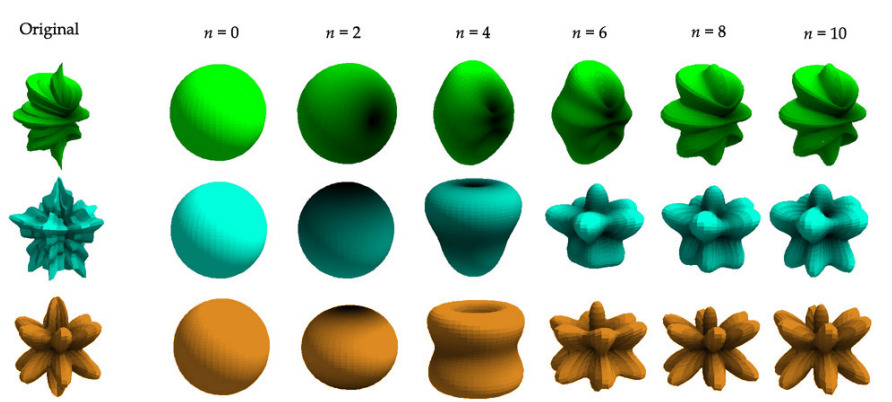
\includegraphics[width=0.6\linewidth]{images/chapter2_img/SHSignalReconstruction.jpg}
        \caption{Ανακατασκευή Σήματος με χρήση σφαιρικών αρμονικών, πηγή \cite{nuajSphericalHarmonicsPortalWakapon}(Robin Green)]}
        \label{fig:SHSignalReconstruction}
    \end{figure}

    Έτσι προκύπτει μια αποδοτική κωδικοποίηση των διανυσμάτων προβολής στα δίκτυα ακτινοβολίας.
    
\subsection{Τρισδιάστατος χωρικός κατακερματισμός- Multi-resolution Hash 3D Encoding}
 Νέες  μέθοδοι αναφέρονται στην κωδικοποίηση έμμεσων αναπαραστάσεων που γενικότερα αναφέρονται και στην βιβλιογραφία ως πρότυπα γραφικών (\enit{Neural Graphics Primitives} \cite{mueller2022instant}). Αυτές, καταδεικνύουν  πως γεωμετρίες έμμεσων πεδίων προσημασμένης απόστασης , ογκομετρικών πεδίων, πεδίων ακτινοβολίας, ακόμα και εικόνων  όταν κωδικοποιούνται με πυρήνες συναρτήσεων που τα αντιστοιχούν σε χώρους μεγαλύτερων διαστάσεων, για να αποτυπώσουν ανώτερες συσχετίσεις των δεδομένων, πρακτικά δημιουργούν δομές που εκπαιδεύονται δύσκολα. Έτσι βασίζονται σε ευριστικά ή δομικά τεχνάσματα που εφαρμόζονται στα δίκτυα κάποια από τα οποία εμφανίζονται στα πλαίσια της θεωρίας ομαλοποίησης και άλλα βασίζονται στην εκμάθηση υπολειπομένων αναπαραστάσεων σε \enit{ResNet}. Αυτό γίνεται μιας και η απόδοση της εκπαίδευσης των δικτύων μειώνεται δραματικά και ο έλεγχος σε δεδομένα υψηλής διάστασης, όπου δεικτοδότηση είναι ακριβή υπολογιστικά, είναι χρονοβόρος και απαιτεί μεγάλο αριθμό πόρων. 
 \par 
    Αυτό καλούνται να λύσουν οι μέθοδοι 3D κωδικοποίησης που κάνουν χωρικό κατακερματισμό σε πολλαπλά επίπεδα ανάλυσης δίνοντας αυτόματα προτεραιότητα σε αραιά χαρακτηριστικά περιοχών και σταδιακά αυξάνοντας την ανάλυση κωδικοποίησης οδηγούν στην εκμάθηση και λεπτομερειών υψηλής ακρίβειας.
\par 
    Μια τέτοια μέθοδος είναι και η κωδικοποίηση κατακερματισμού \enit{Hash Encoding} που εφαρμόζεται σε δίκτυα συντεταγμένων και δημιουργεί χάρτες χαρακτηριστικών σε αυξανόμενες αναλύσεις επιμερίζοντας το πρόβλημα σε απλούστερα υπό προβλήματα τα οποία είναι σε θέση να είναι αποσυσυσχετισμένα μεταξύ τους μιας και επιλέγεται διαδικασία κατακερματισμού που επιτρέπει με χρήση της πράξης XOR(\enit{Exclusive OR}) στις συντεταγμένες και έχει τη δυνατότητα να αποφύγει από μόνη της συμπίπτουσες κωδικοποιημένες συντεταγμένες. 
    \begin{equation*}
        h(\mathbf{x})=\bigoplus_{i=1}^{d}x_{i}\pi_{i}, 
        \label{eq:hashfunction}
    \end{equation*}

    όπου d η διάσταση των δεδομένων στον πίνακα κατακερματισμού και $\pi_i$ διάνυσμα ακεραίων αριθμών, με τις οποίες εφαρμόζεται αποκλειστική διάζευξη σε επίπεδο bit (\enit{Bitwise XOR}). 
\par
    Οι χάρτες κατακερματισμένων χαρακτηριστικών (άτλαντες διαφορίσιμων πολλαπλοτήτων) σε διάφορες αναλύσεις του χώρου έχουν συγκεκριμένο μέγεθος και αντιστοιχίζονται με παρεμβολή (χρήση interpolation στα χαρακτηριστικά κελιών) σε βάρη, όπως εκτελούν και στρώματα προσοχής (\enit{Attention Layers} \cite{vaswani2023attention}).
\par 
    Οι χωρικές ιεραρχίες (\enit{spatial hierarchical encoding}) που εισάγονται με αυτού του τύπου των κωδικοποιήσεων, επιτρέπουν με ίδιο αριθμό παραμέτρων πολύ πιο γρήγορη κωδικοποίηση και εκπαίδευση δίνοντας ανάλογα αποτελέσματα χωρίς να κωδικοποιούνται δύσκολες συσχετίσεις δεδομένων σε υψηλές διαστάσεις. Περισσότερα στην μεθοδολογία Κεφ.\ref{chapter:implementations}.

    
\subsection{ Θυρίδες Κατακερματισμένων φίλτρων Fourier NFFB \cite{wu2023neural}}
    Παρά την επιτυχία της προηγούμενης μεθόδου, παρατηρούνται προβλήματα όταν γίνεται αποκλειστική χρήση χαρτών κατακερματισμού στην εκπαίδευση πεδίων προσημασμένης απόστασης που έχουν να κάνουν με την ποιότητα του αποτελέσματος {εμφανίζονται \enit{artifacts}}. Επομένως μια καλή επιλογή είναι ο συγκερασμός των δύο μεθόδων με το σκεπτικό του μετασχηματισμού κυματιδίων \enit{wavelets}. Αυτό, συνδυάζει τις δυο  παραπάνω μορφές κωδικοποίησης ταυτόχρονα και αρμονικά μεταξύ τους και ονομάζεται Νευρωνικές Θυρίδες κατακερματισμένων Φίλτρων Fourier ή \enit{Neural Fourier Filter Banks} \cite{wu2023neural} τα οποία πλέον αποτελούν τον άτλαντα χαρακτηριστικών των αμφισδιαφορίσιμων πεδίων γεωμετρίας και φωτισμού. 
    
\subsubsection{Μετασχηματισμός Κυματιδίων - Wavelet Transform}
    Η χρήση του μετασχηματισμού κυματιδίων, έχει ερευνηθεί αρκετά στην βιβλιογραφία της βαθιάς μάθησης. Για παράδειγμα, χρησιμοποιούνται για δειγματοληψία χαρακτηριστικών βασισμένη στα κυματίδια (\enit{wavelet-based feature pooling}). Τέτοια διαδικασία, εισάγει βελτιώσεις στο κομμάτι της μεταφοράς χαρακτηριστικών ή στην αποθορυβοποίηση εικόνων για ιατρική ανάλυση. Στο κομμάτι των παραγωγικών-αντιπαραθετικών δικτύων (\enit{GANs}) που γεννούν εικόνες  κάποιες υλοποιήσεις βασίζονται εξολοκλήρου στην αποσύνθεση σημάτων με χρήση μετασχηματισμού κυματιδίων. Άλλες, προτείνουν επαυξημένο διαχωριστή (\enit{discriminator, δομή των \enit{GAN} δικτύων που προσπαθεί να διαχωρίσει τα παραγόμενα από τα πραγματικά δεδομένα}), πάνω στις υποζώνες(\enit{sub bands}) συχνοτήτων που προκύπτουν από έναν μετασχηματισμό κυματιδίων. Η χρήση του λοιπόν είναι σημαντική και μπορεί να εφαρμοστεί στην κωδικοποίηση τρισδιάστατης πληροφορίας με εφαρμογές στην \enit{3D} όραση.
    
    Η ουσία των νευρωνικών θυρίδων Fourier είναι πως λειτουργούν παρόμοια με έναν μετασχηματισμό κυματιδίων.Συγκεκριμένα, γίνεται αναπαράσταση χαρακτηριστικών σε μια κλίμακα κατακερματισμού που επιτρέπει την απόκτηση των πρωτότυπων βαθιών χαρακτηριστικών από μητρικά χαρακτηριστικά μέσω αλλαγής της κλίμακας του χώρου δηλαδή της ανάλυσης του κατακερματισμού. Έτσι αποκτάμε θυρίδες που έχουν χαρακτηριστικά τα οποία μπορούν να αντιστοιχούν σε δεδομένα σε υψηλές διαστάσεις αλλά δεν χρησιμοποιούνται απευθείας στην διαδικασία εκπαίδευσης όπως είναι, με αποτέλεσμα να οδηγούμαστε με μικρές, αλλά ουσιώδης μορφές κωδικοποιήσεων με υψηλή ακρίβεια αναπαραστάσεων χωρίς λανθάνων τεχνουργήματα (\enit{artifacts}).

    Αυτή η διαδικασία αναπαριστάται συμβολικά στις παρακάτω εικόνες που δίνεται η διαφορά στους τρόπους χωρικής/συχνοτικής κωδικοποίησης και πως γίνεται ο συνδυασμός τους.
    
    \begin{figure}[H]
        \centering
        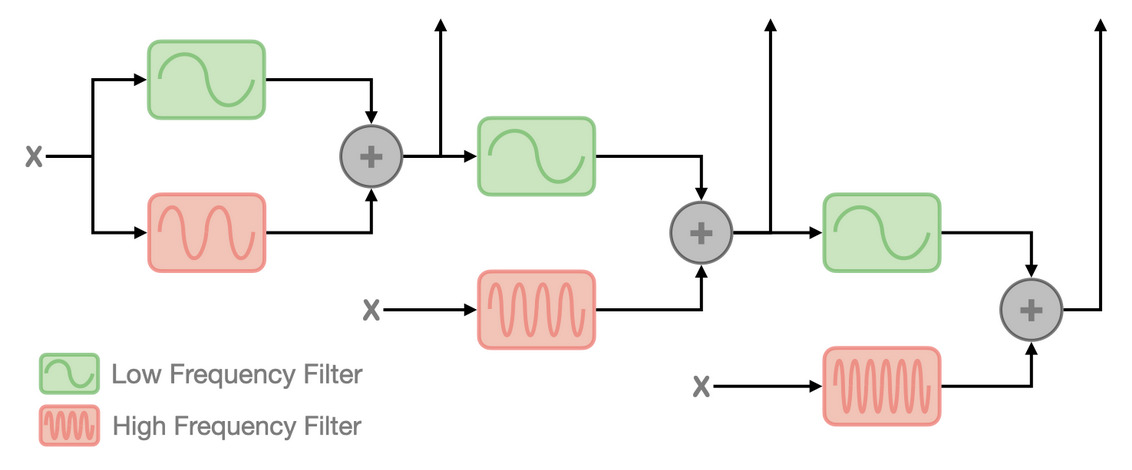
\includegraphics[width=0.8\linewidth]{images/chapter2_img/LowFreqHighFreqNFFBSignalDecomposition.jpg}
        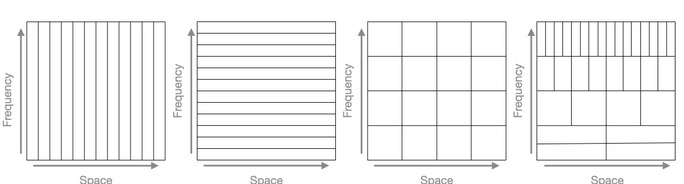
\includegraphics[width=0.8\linewidth]{images/chapter2_img/spatial-frequency_decomposition.jpg}
        \caption{Αναπαράσταση Wavelet κατακερματισμένης κωδικοποίησης υψηλών και χαμηλών συχνοτήτων  σε μια και δύο διαστάσεις με χρήση φίλτρων, πηγή \cite{wu2023neural}}
        \label{fig:nffbdecomp}
    \end{figure}
    \clearpage